\part{Seminar 12 - Optimum design for improving modulating-
effect of coaxial magnetic gear using
response surface methodology and genetic
algorithm}

\makebox[.25\textwidth]{Alexandre Bruliau}\makebox[.25\textwidth]{Miguel Freixo}\makebox[.25\textwidth]{Paolo Thiran}\makebox[.25\textwidth]{Antoine Winant}

\section{Introduction}

This report explain a seminar given in the class of LELEC2311 
\begin{figure}[H]
\centering
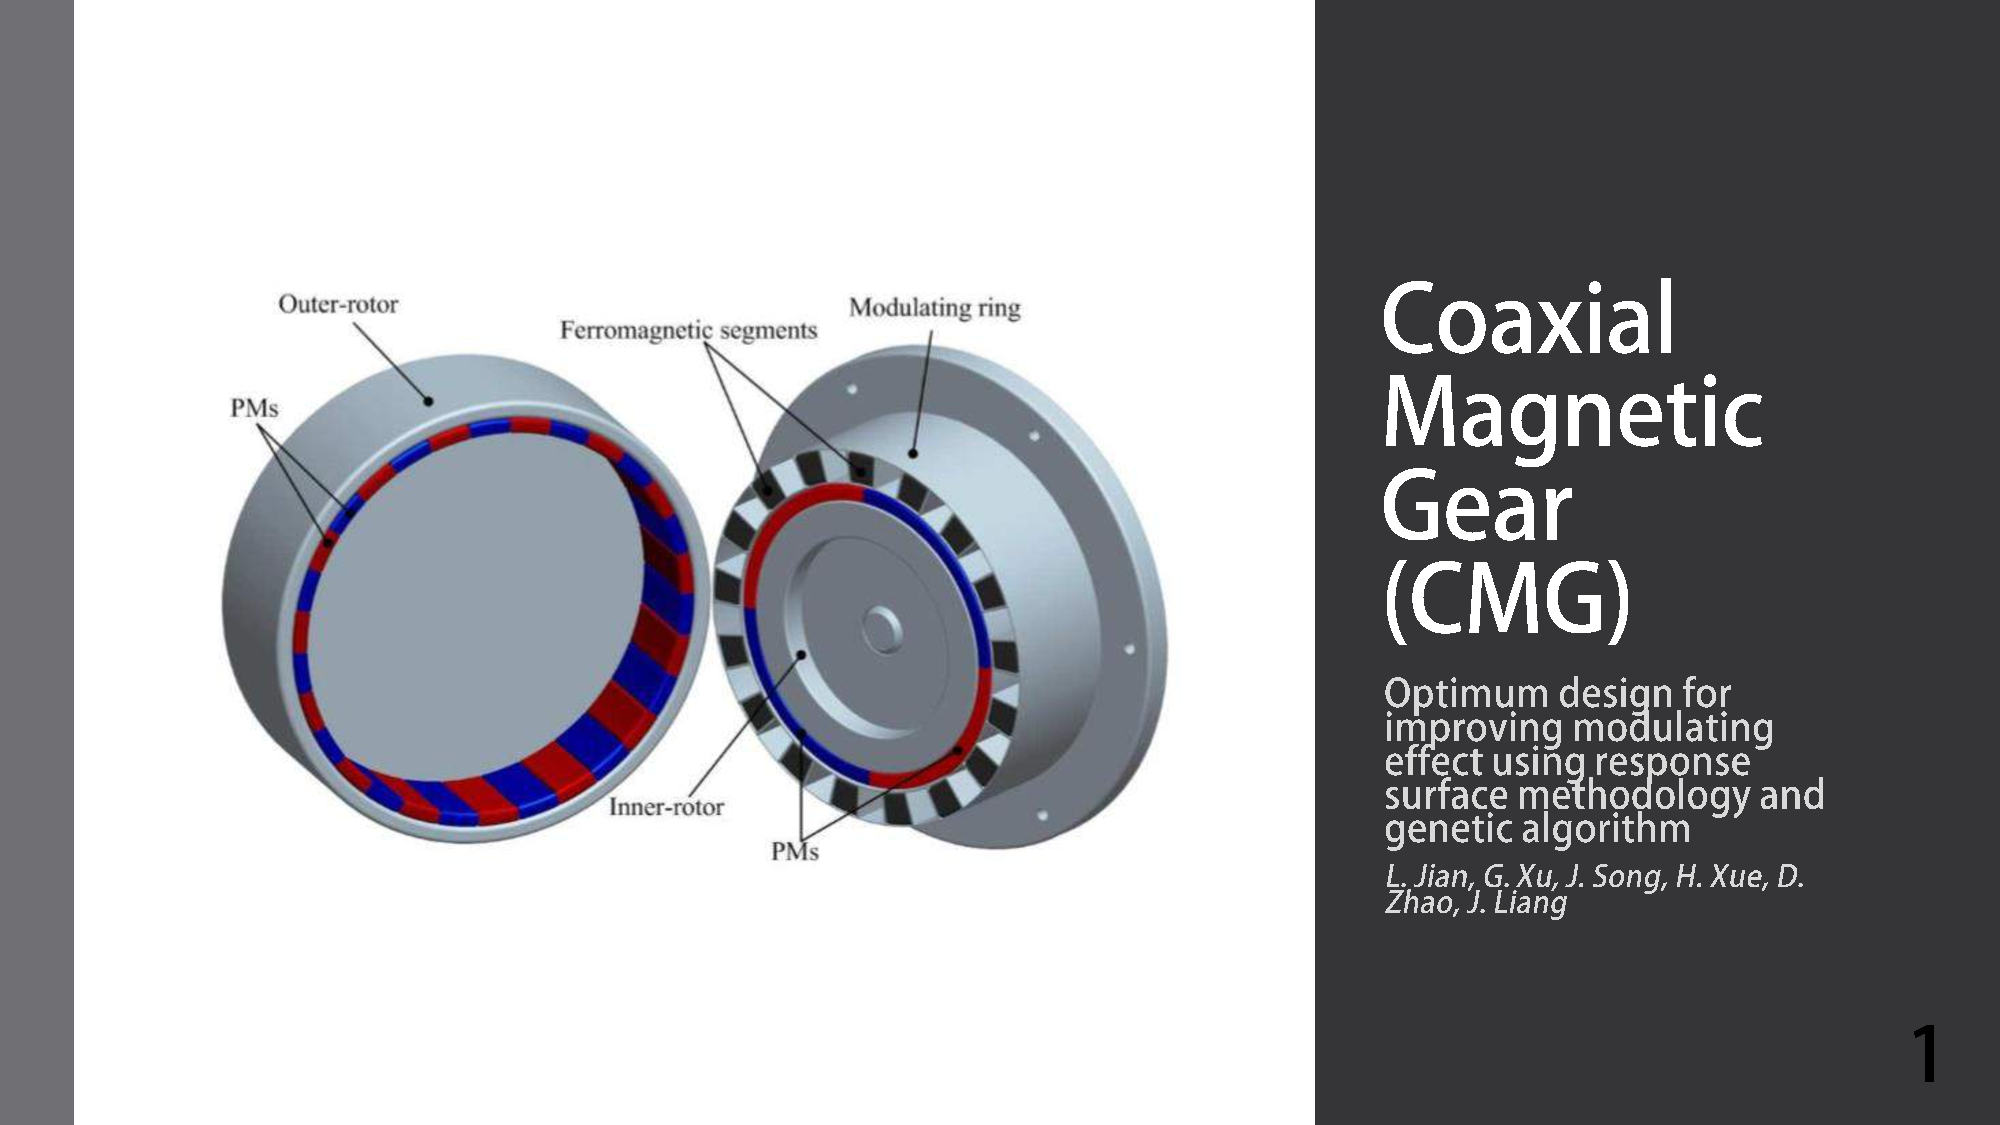
\includegraphics[page={1},scale=0.3]{LELEC2311.pdf}
\caption{First slide}
\label{fig:first slide}
\end{figure}

\section{Context}
\begin{figure}[H]
\begin{minipage}{0.45\linewidth}
CMG can be of interest for applications where we need high reliability.

For instance : 
\begin{itemize}
    \item In the transmission chain of train propulsion, if the mechanical gear gets overloaded, it may break and if it does not break, it will continue to transmit the torque. Because of this, we need to oversize all the downstream elements. On the contrary, with CMG, if it is overloaded, it will just stop transmitting torque. It acts as a protective element and allow to not oversize the rest of the transmission chain.
    \item In oil industry, they have a lot of time and money losses because of mechanical gear breaking. Hence, they are very interested into CMG that might be a more reliable gear and needs less maintenance.
\end{itemize}
\end{minipage}
\hfill
\begin{minipage}[c]{0.45\linewidth}
\centering
\includegraphics[page={2},width=\textwidth]{LELEC2311.pdf}
\label{fig:slide2}
\end{minipage}
\end{figure}

\section{Comparison with mechanical gears}

\begin{figure}[H]
    \begin{minipage}{.45\linewidth}
        
        There is 2 types of magnetic gear: 
        \begin{itemize}
            \item Converted magnetic gears
            \item Field modulated magnetic gears
        \end{itemize}
        
        \paragraph{Converted magnetic gears} also called MGs with ``direct'' effect. Their structures are very similar to that of mechanical gears. We keep the usual topologies but we use permanent magnets rather than gears with teeth.
        
        \paragraph {Field modulated magnetic gears} also called ``flux guided'' MGs. Unlike converted MGs, there is always the presence of a ferromagnetic segment that leads the flux from one gear to another. The role of this segment is very important and it is thanks to him that the 2 rotors can rotate at different speeds. You will understand in the rest of the document why it is necessary to modulate the magnetic field generated by permanent magnets. There are mainly 3 types of field modulated MGs. They are different in their configuration but they work on the same principle. There is the linear type, axial type and coaxial type. The choice of the type depends on the application. if the room in length is restricted, we will use for example an axial or coaxial type.
        
    \end{minipage}
    \hfill%
    \begin{minipage}[c]{.45\linewidth}
        \centering
        \includegraphics[page={6},width=\textwidth]{LELEC2311.pdf}
        \caption{Pictures from Magnetic Gear Technologies: A Review, P.M. Tlali, R-J. Wang, S. Gerber}
    \end{minipage}
\end{figure}


\begin{figure}[H]
    \begin{minipage}{.45\linewidth}
        
        You probably already know all the advantages and defaults of Mechanical gears.
        It can be seen that the disadvantages of mechanical gears are actually the benefits of MGs.
        
        It has no wearing part and therefore does not require oil lubrication, resulting in high reliability and little or no maintenance. The main benefit of MGs is that they don’t break if they are overloaded. This is the main criterion that makes MGs more interesting than mechanical gears in some applications. The physical isolation is also interesting. In fact, in the axial topology, it is possible to pass a sheet of paper between the shafts. 
        The main disadvantage of MGs is that they are expensive because the fabrication process is complex. 
        
        In addition, the axial topology is more complicated to build. Indeed, in the radial topology, the magnets do not attract/repel in average because the forces of attractions/ repulsions are compensated by symmetry. In the axial topology, this is not the case. It is therefore necessary to take care to counter these efforts during fixing.

    \end{minipage}
    \hfill%
    \begin{minipage}[c]{.45\linewidth}
        \centering
        \includegraphics[page={7},width=\textwidth]{LELEC2311.pdf}
    
    \end{minipage}
\end{figure}

\begin{figure}[H]
    \begin{minipage}{.45\linewidth}
        As with any gear, one shaft is rotating at a different speed to the other and the goal is to transmit a torque between those shafts. 
        The gear consists of 3 rings:
        2 (outer and inner) are composed of powerful PM arranged in alternating North-South poles. Between them, the third part is a ferromagnetic ring that creates the \underline{ modulating effect}. (illustrated in a few slide)
        video link: \url{https://www.youtube.com/watch?v=PyBTE5cjGDY}
    \end{minipage}
    \hfill%
    \begin{minipage}[c]{.45\linewidth}
        \centering
        \includegraphics[page={9},width=\textwidth]{LELEC2311.pdf}
    \end{minipage}
\end{figure}

\begin{figure}[H]
    \begin{minipage}{.45\linewidth}
        
       Another view, to make sure you understand well the structure. 
       \begin{itemize}
           \item The inner ring consists of a low number of magnets and is connected to the high speed shaft. 
           \item The middle ring is the modulating ring. It is composed of ferromagnetic parts held in a mechanical structure.
           \item The outer ring consists of a high number of magnets (poles) and in connected to the low-speed shaft. 
       \end{itemize}
       
       Like in a mechanical gear composed of three parts, we can change the gear ratio by choosing which one of the three part is fixed.


    \end{minipage}
    \hfill%
    \begin{minipage}[c]{.45\linewidth}
        \centering
        \includegraphics[page={10},width=\textwidth]{LELEC2311.pdf}
    
    \end{minipage}
\end{figure}

\begin{figure}[H]
    \begin{minipage}{.45\linewidth}
        
       This slide allows to really understand the working principle of the gear and explain how it turns even if the outer and inner rotors have different numbers of poles. 
       
       
       \begin{itemize}
           \item Let’s first look at the field produced by the outer magnets if we neglect the steel segments. It has an array of north/south poles rotating at the same speed (low speed side). 
           \item Now let’s look at the field generated by the outer ring but \underline{after} the modulating ring. The ferromagnetic ring alters/modulates this field pattern. Now as the outer magnetic field rotates, the field has just two Norths and two Souths rotating at a higher speed and in a different direction.
           \item If we place now a inner ring consisting of 2 Norths and 2 Souths, it will couple with this field and rotate at this higher speed. The field generated by the permanent magnets of the inner ring is also modulated, it goes from high speed to lower speed.
       \end{itemize}
       
       That answers the question \textit{“How can the gears rotate if inner/outer shafts have different number of poles"?}


    \end{minipage}
    \hfill%
    \begin{minipage}[c]{.45\linewidth}
        \centering
        \includegraphics[page={11},width=\textwidth]{LELEC2311.pdf}
        \caption{Look at the video to understand well!}
    \end{minipage}
\end{figure}


\begin{figure}[H]
    \begin{minipage}{.45\linewidth}
        
       Here is another representation of the modulating effect. We see clearly the different numbers of poles before and after the stationary pole pieces, on the image with the field lines. 



    \end{minipage}
    \hfill%
    \begin{minipage}[c]{.45\linewidth}
        \centering
        \includegraphics[page={12},width=\textwidth]{LELEC2311.pdf}
    \end{minipage}
\end{figure}

\section{CMG analytical approach}

\begin{figure}[H]
    \begin{minipage}{.45\linewidth}
        \centering
         On the slide 14 you can see the main goal of the approach :
         \begin{itemize}
             \item We want to find the relation between the reduction ration and the poles and the relation between the number of ferromagnetic segment and the number of pair of poles so that it works efficiently.
             \item We want a simple model that proves that harmonics are behind the working principle of magnetic gear.
             \item We want to find the expression of the torque and prove that it is stable.
         \end{itemize}
    \end{minipage}
    \hfill%
    \begin{minipage}[c]{.45\linewidth}
        \centering
        \includegraphics[page={13},width=\textwidth]{LELEC2311.pdf}
    \end{minipage}
\end{figure}

\begin{figure}[H]
    \begin{minipage}{.45\linewidth}
        Here you have a small synthesis of the law that we will use on the next slides to develop the model. Also the assumptions.
    \end{minipage}
    \hfill%
    \begin{minipage}[c]{.45\linewidth}
        \centering
        \includegraphics[page={14},width=\textwidth]{LELEC2311.pdf}
    \end{minipage}
\end{figure}


\begin{figure}[H]
    \begin{minipage}{.45\linewidth}
    
        Introduction to a new concept: surface permeance. The permeance is the inverse of the reluctance. 
        In our case we will consider an infinitesimal tube represented in yellow on the gear such that the flux density is constant inside this tube. Since we take a very small tube we can consider $dS$ as a $\Delta S$ and compute the flux by a product ( $ B.\Delta S$) instead of using the integral. In a certain way we discretize the flux density over small surfaces.
        Taking the formula that links the MMF to the flux : $F = \Phi R$, we can now replace the flux and the reluctance : $F = B \Delta S \frac{h}{\mu_0\Delta S}$ Simplifying by the surface, we obtain $$ F = \frac{ B h}{\mu_0 }  = B R_S $$
        
       The surface reluctance (or surface permeance for the inverse) gives a direct relationship between the magnetomotive force and the flux density inside the magnet 
       
    \end{minipage}
    \hfill%
    \begin{minipage}[c]{.45\linewidth}
        \centering
        \includegraphics[page={15},width=\textwidth]{LELEC2311.pdf}
    \end{minipage}
\end{figure}

\begin{figure}[H]
    \begin{minipage}{.45\linewidth}
        Now all the formulas and the concept were explained. This slide describes the methodology that we will follow to find how the flux is modulated by the ferromagnetic ring. 
        
        \begin{enumerate}
            \item Firt we want to try to find what is the MMF generated by the magnet without the modulation ring.
            \item Then we want to find the expression of the reluctance inside the circuit.
            \item We will find the flux density expression by multiplying the MMF and the permeance find previously
            \item We can derive the torque expression.
        \end{enumerate}
        
    \end{minipage}
    \hfill%
    \begin{minipage}[c]{.45\linewidth}
        \centering
        \includegraphics[page={16},width=\textwidth]{LELEC2311.pdf}
    \end{minipage}
\end{figure}

\begin{figure}[H]
    \begin{minipage}{.45\linewidth}
        We have already obtained an expression that links the MMF to the flux density. We can use it directly if we know how the flux density can be modelise.
        
        On this slide we also use an other definition of the MMF and we obtain at the end the same expression.
    \end{minipage}
    \hfill%
    \begin{minipage}[c]{.45\linewidth}
        \centering
        \includegraphics[page={17},width=\textwidth]{LELEC2311.pdf}
    \end{minipage}
\end{figure}

\begin{figure}[H]
    \begin{minipage}{.45\linewidth}
      We have to make an assumption on the flux density of the permanent magnet. Will consider that it as a cosine expression for the rest of the model.
    \end{minipage}
    \hfill%
    \begin{minipage}[c]{.45\linewidth}
        \centering
        \includegraphics[page={18},width=\textwidth]{LELEC2311.pdf}
    \end{minipage}
\end{figure}

We want now find the permeance of our circuit. Take a slice of the gear as represented on the left picture at the top. We have a slice of PM, gap and either magnetic rods or gap. Thus the permeance varies periodically and looks like a square waves. We can either represent it as a discontinious function or as a Fourier series. We will prefer here the continuous expression to derive the model. It expression is given in the figure on the right. Point 2 of the global methodology done.

$N_s$ is the number of ferromagnetic rods that we place, we do not know how many we need yet but will try to discover it a bit later on.
\begin{figure}[H]
    \begin{minipage}{.45\linewidth}
        \includegraphics[page={20},width=\textwidth]{LELEC2311.pdf}
    \end{minipage}
    \hfill%
    \begin{minipage}[c]{.45\linewidth}
        \centering
        \includegraphics[page={21},width=\textwidth]{LELEC2311.pdf}
    \end{minipage}
\end{figure}


\begin{figure}[H]
    \begin{minipage}{.45\linewidth}
     Point 3, we have the expression of the MMF and the expression of the permeance, using the definition of the MMF we can now compute how the flux density evolves with the permeance. 
     
     The Fourier series (from the permeance) creates all the harmonics that will hopefully interact with one another to create a stable torque. We will be interested only by the fundamental and the first harmonic of each field generated by each magnet.
     
    \end{minipage}
    \hfill%
    \begin{minipage}[c]{.45\linewidth}
        \centering
        \includegraphics[page={23},width=\textwidth]{LELEC2311.pdf}
    \end{minipage}
\end{figure}

\begin{figure}[H]
    \begin{minipage}{.45\linewidth}
        We can now write the equation for each magnet and it will be noted $B_{im}$ for inner magnet and $B_{om}$ for outer magnet. Then $B^0$ is the fundamental and $B^1$ is the first harmonic.
        
        As you can see $N_s$ only appear in the first harmonic and not in the fundamental, thus we can modify only the first harmonic expression by playing with this parameter. So we will try to choose the appropriate value of $N_s$ so that the first harmonic produce by one magnet will interact with the fundamental of the other one. Hopefully the relation  for the other fundamental and first harmonic will also be verified. 
        
        If you wonder why we do not use the to fundamental, it is because there is no way it will have the same number of pair of pole since $N_s$ is not part of this expression.
    \end{minipage}
    \hfill%
    \begin{minipage}[c]{.45\linewidth}
        \centering
        \includegraphics[page={24},width=\textwidth]{LELEC2311.pdf}
    \end{minipage}
\end{figure}

\begin{figure}[H]
    \begin{minipage}{.45\linewidth}
        Using trigonometry we can transform the expression of the first harmonic and the product become a sum.
        
        In one hand we can identify on part of the sum with the expression of the fundamental of the other magnet.
        
        On the other hand we have a other term that will not contributes to the transmission and we do not want it (just forget it) 
    \end{minipage}
    \hfill%
    \begin{minipage}[c]{.45\linewidth}
        \centering
        \includegraphics[page={25},width=\textwidth]{LELEC2311.pdf}
    \end{minipage}
\end{figure}

\begin{figure}[H]
    \begin{minipage}{.45\linewidth}
        If the two components have to interact in a stable way, they have to have the same spatial distribution and the same variation in time. Thus we equals those terms together and we find two conditions. The numbers of magnetic segment is given by the sum of the number of pair of poles. The reduction ratio is given by the ratio.
    \end{minipage}
    \hfill%
    \begin{minipage}[c]{.45\linewidth}
        \centering
        \includegraphics[page={26},width=\textwidth]{LELEC2311.pdf}
    \end{minipage}
\end{figure}

  The two slides are recap slide defining useful parameters. 
\begin{figure}[H]
    \begin{minipage}{.45\linewidth}
       \includegraphics[page={27},width=\textwidth]{LELEC2311.pdf}
    \end{minipage}
    \hfill%
    \begin{minipage}[c]{.45\linewidth}
        \centering
        \includegraphics[page={28},width=\textwidth]{LELEC2311.pdf}
    \end{minipage}
\end{figure}

\begin{figure}[H]
    \begin{minipage}{.45\linewidth}
       Be careful if you want more information and that you read the paper. The computation of the torque is false. The assumption was made earlier that the flux density was purely radial, however they approach to calculate the torque here is based on Maxwell tensor. To find a torque by this approach, one should consider the axial component thus it is not possible. The proper way to find the torque is by doing an energetic approach with the co-energy.
    \end{minipage}
    \hfill%
    \begin{minipage}[c]{.45\linewidth}
        \centering
        \includegraphics[page={30},width=\textwidth]{LELEC2311.pdf}
    \end{minipage}
\end{figure}

\begin{figure}[H]
    \begin{minipage}{.45\linewidth}
        When we compute the torque we can compute the torque on three component. One can observe that the torque is influenced by the number of pole, the shape factor, the magnet and the load angle. 
        
        The stall torque is when the load angle reaches 90 degrees. At this moment is the torque is greater then the gear will not transmit it anymore and this is the self protecting property.
        
        There are three torque but generally on a the 3 component is fixed while the other rotates, thus there the input torque and the output torque which can be compute with the reduction ratio because the overall power is conserved. The fix component also feels a torque but it is not an useful torque it the reaction force due to Newton action-reaction principle. 
    \end{minipage}
    \hfill%
    \begin{minipage}[c]{.45\linewidth}
        \centering
        \includegraphics[page={31},width=\textwidth]{LELEC2311.pdf}
    \end{minipage}
\end{figure}

\section{Analysis of the Harmonics}
\begin{figure}[H]
    \begin{minipage}{.45\linewidth}
    On the left on the slide, we can observe that the evolution of the flux in the radial direction follow a perfect 4 pair pole sinusoidal wave due to the inner rotor (in dotted line). When we add the ferromagnetic pole pieces, harmonics with a higher order are added to the fundamental one.
    On the right of the slide, we observe that for p=4 , the fundamental is the highest harmonic and an other harmonic appear ( with p=22) to interact with the outer rotor. We can verify it by making sure the speed of this harmonic is the same as the speed of the outer ring.
       
    \end{minipage}
    \hfill%
    \begin{minipage}[c]{.45\linewidth}
        \centering
        \includegraphics[page={33},width=\textwidth]{LELEC2311.pdf}
        \caption{33 th slide}
        \label{fig:33_th slide}
    \end{minipage}
\end{figure}

\begin{figure}[H]
    \begin{minipage}{.45\linewidth}
    We can do an analog reasoning as the previous case except that we look at the inner air gap. And so the fundamental one is for p = 22 and the harmonic modulated is for p = 4, it will interact with the inner rotor.(We can verify their speed are equals).
       
    \end{minipage}
    \hfill%
    \begin{minipage}[c]{.45\linewidth}
        \centering
        \includegraphics[page={34},width=\textwidth]{LELEC2311.pdf}
        \caption{34 th slide}
    \end{minipage}
\end{figure}

\begin{figure}[H]
    \begin{minipage}{.45\linewidth}
    We discuss the result of another paper to better understand the impact of the modulating rotor. It is the same reasoning as the 33th slide except a different number of pole on the outer rotor.
       
    \end{minipage}
    \hfill%
    \begin{minipage}[c]{.45\linewidth}
        \centering
        \includegraphics[page={35},width=\textwidth]{LELEC2311.pdf}
        \caption{35 th slide}
    \end{minipage}
\end{figure}

\begin{figure}[H]
    \begin{minipage}{.45\linewidth}
    On the right, we observe that when we add the middle ring, new harmonic will appear and an asynchronous harmonic for p=10 produced by the inner rotor will interact with the fundamental one of the outer rotor and will produce efficient torque.
 
       
    \end{minipage}
    \hfill%
    \begin{minipage}[c]{.45\linewidth}
        \centering
        \includegraphics[page={36},width=\textwidth]{LELEC2311.pdf}
        \caption{36 th slide}
    \end{minipage}
\end{figure}

\begin{figure}[H]
    \begin{minipage}{.45\linewidth}
    When we gather now the inner + outer rotor +ferromagnetic pieces, we can observe, in the outer air gap, that the harmonic for p=10 result in the fundamental one produce by the outer rotor and an other harmonic modulated by the inner rotor(witch has the same pair pole number)
 
       
    \end{minipage}
    \hfill%
    \begin{minipage}[c]{.45\linewidth}
        \centering
        \includegraphics[page={37},width=\textwidth]{LELEC2311.pdf}
        \caption{37 th slide}
    \end{minipage}
\end{figure}

\begin{figure}[H]
    \begin{minipage}{.45\linewidth}
    We can do an analog reasoning for the previous slide except that we look from the inner air gap. And so, the harmonic for p=4 result in the fundamental one produce by the inner rotor and an other harmonic modulated by the outer rotor.
 
       
    \end{minipage}
    \hfill%
    \begin{minipage}[c]{.45\linewidth}
        \centering
        \includegraphics[page={38},width=\textwidth]{LELEC2311.pdf}
        \caption{38 th slide}
    \end{minipage}
\end{figure}

\begin{figure}[H]
    \begin{minipage}{.45\linewidth}
    A good advantage is that a large part of fluxlines can pass through the two air gaps thanks to the very low reluctance of the ferromagnetic pole pieces. These fluxline will contribute efficiently to the torque.

 A first drawback of this machine is that there is some flux leakeage due to the interaction between 2 PM that will not be take into account in the efficient torque transmission.
 
       
    \end{minipage}
    \hfill%
    \begin{minipage}[c]{.45\linewidth}
        \centering
        \includegraphics[page={39},width=\textwidth]{LELEC2311.pdf}
        \caption{39 th slide}
    \end{minipage}
\end{figure}

\begin{figure}[H]
    \begin{minipage}{.45\linewidth}
    The reluctant torque that comes from the interaction between the inner / outer ring is the efficient torque. Howver, a cogging torque that induce ripple will decreases the performance of the CMG.
    On the left of the slide, we can see the torque on the inner rotor (by blocking the outer rotor and rotating incrementally this one). When it achieves its maximum , that means the total field B produce by the inner rotor is offset by $90 \degree$ respecting to the outer rotor. When we look at the harmonics, it will produce efficient torque for p = 4 but some parasitic harmonic are also present for p = 56 (ripple harmonic). We can find them by computing the ppcm between the number of pole on the outer / inner rotor and the number of pole pieces.

 
       
    \end{minipage}
    \hfill%
    \begin{minipage}[c]{.45\linewidth}
        \centering
        \includegraphics[page={40},width=\textwidth]{LELEC2311.pdf}
        \caption{40 th slide}
    \end{minipage}
\end{figure}

\begin{figure}[H]
    \begin{minipage}{.45\linewidth}
   We can do a similar reasoning for the ripple torque on the outer rotor.
   When we look at the harmonics, it will produce efficent torque for p = 10 but some parasitic harmonic are also present for p = 140 (ripple harmonic). We can find them by computing the ppcm as we explained it before.

 
       
    \end{minipage}
    \hfill%
    \begin{minipage}[c]{.45\linewidth}
        \centering
        \includegraphics[page={41},width=\textwidth]{LELEC2311.pdf}
        \caption{41 th slide}
    \end{minipage}
\end{figure}

\begin{figure}[H]
    \begin{minipage}{.45\linewidth}
   A factor called the cogging factor allow us to characterize this cogging torque. Basically we would like to minimize it (almost equal to 1) to reduce the ripple. To do that we can use the time table on the left of the slide. It gives us , for a gear ratio fixed, the cogging factor in function of the number of pole on the inner rotor.

 
       
    \end{minipage}
    \hfill%
    \begin{minipage}[c]{.45\linewidth}
        \centering
        \includegraphics[page={42},width=\textwidth]{LELEC2311.pdf}
        \caption{42 th slide}
    \end{minipage}
\end{figure}


\begin{figure}[H]
    \begin{minipage}{.45\linewidth}
    So far , we have discussed about the CMG where the magnets are mounted in surface. We have seen it was quite working well but still suffer from several drawback : low torque density, high ripple and some iron losses.
    One must know they exist other types : the first one is the second type. The principle is the same of the CMG except the ordering of the PM on the outer / inner rotor. They put them like this (1 ferromagnetic piece between two inverted PM ) to concentrate the flux in the air gap and so to increase the torque density. But it  doesn't solve the problem that we have still some flux leakages. That's why we introduce you the Halbach array.
       
    \end{minipage}
    \hfill%
    \begin{minipage}[c]{.45\linewidth}
        \centering
        \includegraphics[page={44},width=\textwidth]{LELEC2311.pdf}
        \caption{44 th slide}
    \end{minipage}
\end{figure}

\begin{figure}[H]
    \begin{minipage}{.45\linewidth}
    
The principle is the same of the CMG except that these configuration will improve the performance.
The arrow of each PM points towards the magnetic north. They choosed different configuration of the PM for the inner and the outer rotor.
Basically, the configuration will allow a much more sinusoidal flux in the air gap, and so the ripple harmonic will be reduce. As you can see on the bottom of the slide , the field will be amplified in the air gap and will be diminished outside the machine. So we are protected against external magnetic field.
 
       
    \end{minipage}
    \hfill%
    \begin{minipage}[c]{.45\linewidth}
        \centering
        \includegraphics[page={45},width=\textwidth]{LELEC2311.pdf}
        \caption{45 th slide}
    \end{minipage}
\end{figure}




\begin{figure}[H]
    \begin{minipage}{.45\linewidth}
    The choice of the number of segments per pole result in a trade-off: either you decide to increase it and so you will get more torque / flux density but the price will be much higher. In this paper they choosed a different value of the NSP because it will result in a different strength in the magnetic field.
    \end{minipage}
    \hfill%
    \begin{minipage}[c]{.45\linewidth}
        \centering
        \includegraphics[page={46},width=\textwidth]{LELEC2311.pdf}
        \caption{46 th slide}
    \end{minipage}
\end{figure}


\begin{figure}[H]
    \begin{minipage}{.45\linewidth}
    To compute the magnetic field into the air gap : they used the principle of superposition . First, they will compute the field due to only the inner magnet and the outer magnet without the ferromagnetic pieces. After they add it, they will compute the field in the inner air gap, due to the field of the inner magnet a the modulated field from the outer magnet. We can do the inverse way to compute the field in the outer air gap.
    \end{minipage}
    \hfill%
    \begin{minipage}[c]{.45\linewidth}
        \centering
        \includegraphics[page={47},width=\textwidth]{LELEC2311.pdf}
        \caption{47 th slide}
    \end{minipage}
\end{figure}


\begin{figure}[H]
    \begin{minipage}{.45\linewidth}
    We observe that as we said before, we exhibit much lower flux in the outer and inner rotor yoke. Thus they can be reduce ( their inertia, weight) and this might increase the performance (will see later ).
    \end{minipage}
    \hfill%
    \begin{minipage}[c]{.45\linewidth}
        \centering
        \includegraphics[page={48},width=\textwidth]{LELEC2311.pdf}
        \caption{48 th slide}
    \end{minipage}
\end{figure}

\begin{figure}[H]
    \begin{minipage}{.45\linewidth}
   When we compare the radial flux density on the inner air gap of the CMG and the one with the halbach array (HPMG), we noticed indeed, we obtain a much more sinusoidal flux and we can achieve a higher flux in the HPMG.
    \end{minipage}
    \hfill%
    \begin{minipage}[c]{.45\linewidth}
        \centering
        \includegraphics[page={49},width=\textwidth]{LELEC2311.pdf}
        \caption{49 th slide}
    \end{minipage}
\end{figure}

\begin{figure}[H]
    \begin{minipage}{.45\linewidth}
   We will only analyse the harmonics for radial component (because it is the same reasoning for the tangential one) in the inner air gap.
   The pole pair number p = 4 and p = 17 produce by the outer rotor and modulated by the r
 g will contribute efficiently to the transmission of the torque. To find them, you can use the formula we have written. And you can also verify that these harmonics will have the same speed of the inner rotor. Others harmonics are source of ripple( produced by the inner rotor) and sources of iron losses (produced by the outer rotor that will turn at the same speed of the inner rotor but they don't have the same number of pair poles). You can notice that a larg part of these parasitic harmonic will be suppressed in the HPGM.
   It is the same reasoning for the outer air gap.   \end{minipage}
    \hfill%in
    \begin{minipage}[c]{.45\linewidth}
        \centering
        \includegraphics[page={50},width=\textwidth]{LELEC2311.pdf}
        \caption{50 th slide}
    \end{minipage}
\end{figure}

\begin{figure}[H]
    \begin{minipage}{.45\linewidth}
  We can observe the torque on the inner or in the outer rotor is $13 \%$ higher in the HPGM than in the CMG. There is also a difference of $\pi$ between the 2 torques because the turn in the opposite way.
    \end{minipage}
    \hfill%
    \begin{minipage}[c]{.45\linewidth}
        \centering
        \includegraphics[page={52},width=\textwidth]{LELEC2311.pdf}
        \caption{52 th slide}
    \end{minipage}
\end{figure}


\begin{figure}[H]
    \begin{minipage}{.45\linewidth}
  We can observe the ripple torque on the inner rotor is $67 \%$ lower in the HPGM than in the CMG. 
    \end{minipage}
    \hfill%
    \begin{minipage}[c]{.45\linewidth}
        \centering
        \includegraphics[page={53},width=\textwidth]{LELEC2311.pdf}
        \caption{53 th slide}
    \end{minipage}
\end{figure}


\begin{figure}[H]
    \begin{minipage}{.45\linewidth}
  There are 2 types of losses : the iron that comes from the eddy current and the hysteresis of the PM and the stray losses that comes from the resistivity of the materials. But the iron losses are the most important one.
  We can observer the losses plotted in function of the inner speed , in the inner / outer rotor yoke, in the ferromagnetic pieces and in the total machine. And in each of these cases, the losses are always lower in the HPGM than in the CMG
    \end{minipage}
    \hfill%
    \begin{minipage}[c]{.45\linewidth}
        \centering
        \includegraphics[page={54},width=\textwidth]{LELEC2311.pdf}
        \caption{54 th slide}
    \end{minipage}
\end{figure}

\section{Optimization of the shape factors}

\begin{figure}[H]
    \begin{minipage}{.45\linewidth}
    Now that we have understood how the CMG works, we will try to optimize the shape factors of the ferromagnetic segments : $h_s$, $\theta_{down}$ and $\theta_{up}$.
    
    To do that, we will use a surrogate model developped thanks to RSM. It is a good compromise between 1-D analytical model and Finite Element Method.
    \end{minipage}
    \hfill%
    \begin{minipage}[c]{.53\linewidth}
        \centering
        \includegraphics[page={56},width=\textwidth]{LELEC2311.pdf}
        \label{fig:56_th slide}
        \caption{}
    \end{minipage}
\end{figure}

\begin{figure}[H]
    \begin{minipage}{.45\linewidth}
    \textbf{Attention :} error in the table from the paper in figure \ref{fig:57_th slide}
    on the last line it should be $\theta_{down}/x_3$.
    \end{minipage}
    \hfill%
    \begin{minipage}[c]{.53\linewidth}
        \centering
        \includegraphics[page={57},width=\textwidth]{LELEC2311.pdf}
        \caption{}
        \label{fig:57_th slide}
    \end{minipage}
\end{figure}

\begin{figure}[H]
    \begin{minipage}{.45\linewidth}
    How it works to find our second order model with RSM : 
    \begin{itemize}
        \item We make a FEM évaluation of the maximal pull-out torque for a set of n point ($n>15$)
            \begin{itemize}
                \item On the left graph of figure \ref{fig:58_th slide}, we can see the surface corresponding to $T_{max} = f(\theta_{up},\theta_{down})$ and with $h_s = cst$.
                \item On the right graph of figure \ref{fig:58_th slide}, we can see the surface corresponding to $T_{max} = f(\theta, h_s)$ with $\theta  = \theta_{up} = \theta_{down}$.
                \item On both surfaces each summit corresponds to a point of evaluation of $T_{max}$ (thos sufaces are not the meshes of the FEM!!)
            \end{itemize}
        \item We take a subset of m<n evaluation (in this study m = 15) to compute the $\beta$ coefficient of our second order model
        \item Once we have the model, we test it with an analysis-of-variance (ANOVA). We use as a reference for this test the set of n points calculated at the first step.
    \end{itemize}
    \end{minipage}
    \hfill%
    \begin{minipage}[c]{.53\linewidth}
        \centering
        \includegraphics[page={58},width=\textwidth]{LELEC2311.pdf}
        \caption{}
        \label{fig:58_th slide}
    \end{minipage}
\end{figure}

\begin{figure}[H]
    \begin{minipage}{.48\linewidth}
    \centering
        \includegraphics[page={59},width=\textwidth]{LELEC2311.pdf}
    \end{minipage}
    \hfill%
    \begin{minipage}[c]{.48\linewidth}
        \centering
        \includegraphics[page={60},width=\textwidth]{LELEC2311.pdf}
        \label{fig:60_th slide}
    \end{minipage}
    \caption{Comparison between the second-order model found and the FEM evaluation}
\end{figure}


\begin{figure}[H]
    \begin{minipage}{.45\linewidth}
    Once they have developped their model, they choose to optimize it with genetic methods \footnote{That is stupid as the model found is a second order fonction, we could just derive it and find the optimum way faster.}
    The working priciple is described in the figure \ref{fig:61_th slide}. When we say others undergo an operation, it can be or mutation or crossover.
    \end{minipage}
    \hfill%
    \begin{minipage}[c]{.53\linewidth}
        \centering
        \includegraphics[page={61},width=\textwidth]{LELEC2311.pdf}
        \caption{}
        \label{fig:61_th slide}
    \end{minipage}
\end{figure}

\begin{figure}[H]
    \begin{minipage}{.48\linewidth}
    \centering
        \includegraphics[page={62},width=\textwidth]{LELEC2311.pdf}
    \end{minipage}
    \hfill%
    \begin{minipage}[c]{.48\linewidth}
        \centering
        \includegraphics[page={63},width=\textwidth]{LELEC2311.pdf}
        \label{fig:63_th slide}
    \end{minipage}
    \caption{Results of the optimization procedure and conclusion of the presentation}
\end{figure}

In the table of the results of the optimization procedure, we see that the $T_{max}$ found with the model is not exactly the same as the one we get when we compute that point with FEM but is very close. In order to be sure of our results, we could do some more computation with FEM of surrounding points in each direction to see if we really are at a maximum.
